\chapter{Parte di Ruggero}

\section{Background}
This projects has the goal to teach an agent how to get out of a maze. The maze is a simple 5x5 size grid, without obstacles inside.
The agent's starting position is in the lower left corner of the grid while the target position is in the upper right corner. The q-learning technique is used in order to make the agent learn how to get out of the maze. Also, for balancing the exploration and exploitation of the agent, the GLIE method is used. 

\section{Implementation}

\subsection{Enviorment}
The enviorment is imported from the \textit{Open AI Gym}'s libraries and is composed by a 5x5 size grid. Every position defines a state and some action are available in every state.
There are 4 actions available in this environment: up, down, left, right.
The position outside the grid are considered "\textit{out of bounds}" and if an action leads to an out of bounds position, then the move is said \textit{invalid} and a negative reward is provided to that pair \textit{<state, action>}.
If the action is valid, that is, it ends in a state that falls within the limits of the grid, then the agent changes position and will go to the cell indicated by the pair \textit{<state, action>} and will receive a predefined reward. 

\subsection{Reward}
For the 5x5 size grid, our target state is the cell with coordinates (4,4) (that is the opposite corner to that of the agent's starting position). Reaching the target state provides a reward of +10000 while doing an action that would take the agent out of the boundaries of the grid provides a reward of -100. 
In all other cases (the agent is brought into a valid state) the reward is calculated as follows: $new_target_distance = np.linalg.norm(self.state - self.target_state)$. That is, if the distance of the current state from the target state is smaller than the distance of the previous state from the target state (so the agent is getting closer to the goal), then the reward is positive +1, otherwise (so the agent is moving away) negative -1. \\

\section{Learning phase}
The learning of the agent is done in \textit{episodes} and each episode has a certain length ($ env.path_length$) which is measured by the number of actions done by the agent.
The agent, at each step, can decide whether to make an \textit{exploitation} or \textit{expoloration} move. This decision is made based on the \textit{epsilon} probability which is calculated according to the \textit{GLIE} methodology: 

$epsilon = 1 / env.path_length$. \\ 
\textbf{IF} $random.uniform(0, 1) < epsilon $\\
\textbf{THEN}  \\
EXPLORE: select a random action \\ 
\textbf{ELSE}\\
EXPLOIT: select the action with max value (best future reward) \\

Each episode starts with $env.path_length$ equal to 1, so the first few moves will have a high chance of being exploratory (and therefore random). As the episode progresses, and therefore the value of $env.path_length$ grows, the likelihood of the agent taking an exploitation action increases.

For each action performed (that is at every step) the variable $env.path_length$ is increased by 1 and a Q-VALUE is associated to the pair $<action, state>$. 
In every moment, the agent is in a certain state (that is a position) and when an action (that is a move) is done, the agent changes position and goes in a new state. Then, the Q-value table is update with the following formula: $ Q_table[state, action] += learning_rate * (reward + gamma * np.max(Q_table[new_state]) - Q_table[state, action])$. 

\begin{figure}[h!]
	\centering
	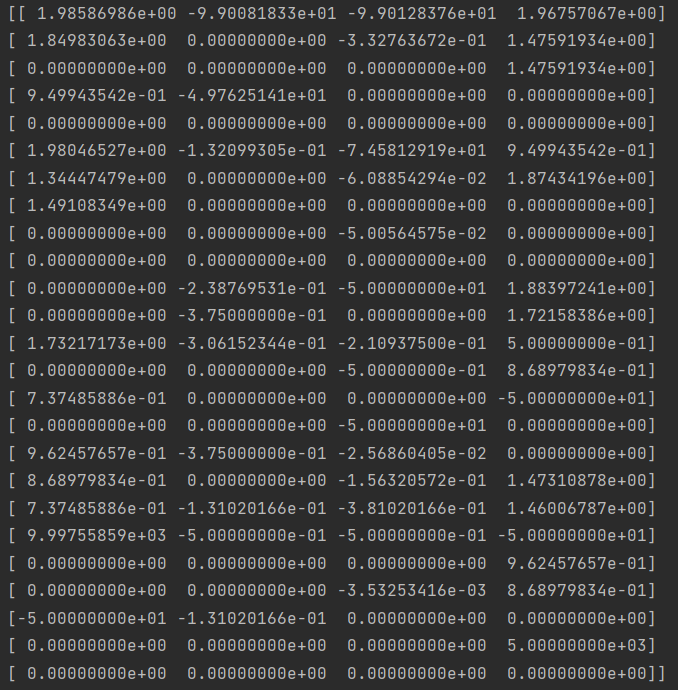
\includegraphics[scale=0.9]{imgs/q-table output.png}
	\caption{Q-table after some episodes: each row represent a state (a 5x5 size grid has 25 states) while the columns represent the 4 possible action in every state. Every pair $<state, action>$ has a value: if in the whole run, an action is not performed in a state then that pair will have value 0. Otherwise the value is given by the q-value update formula.}
	\label{fig:q-}
\end{figure}

The actual learning is done with some \textit{'runs'}. Each run consists of 500 episodes, each one 200 steps long. Each run has a \textit{Q-table} which is updated at each step of each episode. The runs differ in the values of learning rate and gamma, in order to find the optimal combination. At the end of each \textit{run} we should obtain a Q-table containing the values that allow to reach the target state easily (not optimal, not having a reference policy).

An example of Q-table output is shown in \ref{fig:q-}.

\section{Testing Phase}
From the \textit{Learning phase} of the agent we have obtained a \textit{Q-table} for each pair of \textit{Learning Rate} and \textit{Gamma} values which are fed into the \textit{Testing phase}.
In the \textit{Testing phase} the agent always executes the action with the highest q-value (no exploration), thus obtaining a deterministic behavior. This allows us to run a single test for each Q-table.

The testing phase aims to find out what are the optimal values of \textit{learning rate} and \textit{gamma}. The strategy we used to determine which parameter to use to evaluate the $<lr, gamma>$ pair is as follows: if the agent reaches the target state, then the number of \textit{steps} it took to reach it is taken as a parameter, the total \textit{score} otherwise.


\section{Conclusion}
The goal of this task was to teach an agent how to get out of a space (very simple, without obstacles). To do this, it was decided to use the \textit{reinforcment learning} method together with the \textit{GLIE} technique.
This last technique is in my opinion "improvable", that is, it can be implemented in different ways to obtain a better result. 
The problem with standard implementation is that only after a few steps does the probability of exploration drop significantly (after only 10 steps we have a 10\% chance of making an exploration move) and therefore we have a long-tail distribution. 
An improvement would be to divide the episodes of the training phase into two parts: in the first part we use $1 - epsilon$ (so at the beginning of the episodes there will be a high probability of making exploratory moves) while in the second part of the episodes we only use $epsilon$. In this way there will be the possibility to make exploratory moves even towards the end of the episode.

Another interesting approach  could be to make a smoothing in order to linearize the probability distribution.